\documentclass{article}

% if you need to pass options to natbib, use, e.g.:
%     \PassOptionsToPackage{numbers, compress}{natbib}
% before loading neurips_2025

% The authors should use one of these tracks.
% Before accepting by the NeurIPS conference, select one of the options below.
% 0. "default" for submission
\usepackage[dblblindworkshop]{neurips_2025}
% the "default" option is equal to the "main" option, which is used for the Main Track with double-blind reviewing.
% 1. "main" option is used for the Main Track
%  \usepackage[main]{neurips_2025}
% 2. "position" option is used for the Position Paper Track
%  \usepackage[position]{neurips_2025}
% 3. "dandb" option is used for the Datasets & Benchmarks Track
 % \usepackage[dandb]{neurips_2025}
% 4. "creativeai" option is used for the Creative AI Track
%  \usepackage[creativeai]{neurips_2025}
% 5. "sglblindworkshop" option is used for the Workshop with single-blind reviewing
 % \usepackage[sglblindworkshop]{neurips_2025}
% 6. "dblblindworkshop" option is used for the Workshop with double-blind reviewing
%  \usepackage[dblblindworkshop]{neurips_2025}

% After being accepted, the authors should add "final" behind the track to compile a camera-ready version.
% 1. Main Track
 % \usepackage[main, final]{neurips_2025}
% 2. Position Paper Track
%  \usepackage[position, final]{neurips_2025}
% 3. Datasets & Benchmarks Track
 % \usepackage[dandb, final]{neurips_2025}
% 4. Creative AI Track
%  \usepackage[creativeai, final]{neurips_2025}
% 5. Workshop with single-blind reviewing
%  \usepackage[sglblindworkshop, final]{neurips_2025}
% 6. Workshop with double-blind reviewing
%  \usepackage[dblblindworkshop, final]{neurips_2025}
% Note. For the workshop paper template, both \title{} and \workshoptitle{} are required, with the former indicating the paper title shown in the title and the latter indicating the workshop title displayed in the footnote.
% For workshops (5., 6.), the authors should add the name of the workshop, "\workshoptitle" command is used to set the workshop title.
% \workshoptitle{WORKSHOP TITLE}

% "preprint" option is used for arXiv or other preprint submissions
 % \usepackage[preprint]{neurips_2025}

% to avoid loading the natbib package, add option nonatbib:
%    \usepackage[nonatbib]{neurips_2025}

\usepackage[utf8]{inputenc} % allow utf-8 input
\usepackage[T1]{fontenc}    % use 8-bit T1 fonts
\usepackage{hyperref}       % hyperlinks
\usepackage{url}            % simple URL typesetting
\usepackage{booktabs}       % professional-quality tables
\usepackage{amsfonts}       % blackboard math symbols
\usepackage{nicefrac}       % compact symbols for 1/2, etc.
\usepackage{microtype}      % microtypography
\usepackage{xcolor}         % colors

% Custom packages
\usepackage{graphicx}
\usepackage{amsmath}

\workshoptitle{Efficient Reasoning}

% Note. For the workshop paper template, both \title{} and \workshoptitle{} are required, with the former indicating the paper title shown in the title and the latter indicating the workshop title displayed in the footnote. 
\title{Formatting Instructions For NeurIPS 2025 }


% The \author macro works with any number of authors. There are two commands
% used to separate the names and addresses of multiple authors: \And and \AND.
%
% Using \And between authors leaves it to LaTeX to determine where to break the
% lines. Using \AND forces a line break at that point. So, if LaTeX puts 3 of 4
% authors names on the first line, and the last on the second line, try using
% \AND instead of \And before the third author name.


\author{%
  David S.~Hippocampus\thanks{Use footnote for providing further information
    about author (webpage, alternative address)---\emph{not} for acknowledging
    funding agencies.} \\
  Department of Computer Science\\
  Cranberry-Lemon University\\
  Pittsburgh, PA 15213 \\
  \texttt{hippo@cs.cranberry-lemon.edu} \\
  % examples of more authors
  % \And
  % Coauthor \\
  % Affiliation \\
  % Address \\
  % \texttt{email} \\
  % \AND
  % Coauthor \\
  % Affiliation \\
  % Address \\
  % \texttt{email} \\
  % \And
  % Coauthor \\
  % Affiliation \\
  % Address \\
  % \texttt{email} \\
  % \And
  % Coauthor \\
  % Affiliation \\
  % Address \\
  % \texttt{email} \\
}


\begin{document}


\maketitle


\begin{abstract}
  The abstract paragraph should be indented \nicefrac{1}{2}~inch (3~picas) on
  both the left- and right-hand margins. Use 10~point type, with a vertical
  spacing (leading) of 11~points.  The word \textbf{Abstract} must be centered,
  bold, and in point size 12. Two line spaces precede the abstract. The abstract
  must be limited to one paragraph.
\end{abstract}


\section{Introduction}
Large Language Models (LLMs) go through multiple steps of training before reaching a usable state. An LLMs goes through pre-training where it absorbs crucial and basic knowledge of what word comes after a context, then undergoes a finetuning to become a conversational Language Model able to exchange and offer follow-up responses. Finally, it undertakes a preference tuning step where it changes its responses based on human preference. This step is widely uses Reinforcement Learning from Human Feedback (RLHF) algorithms where the models learn from feedback predefined by a human. The way the human feedback is stored and used differs from one RLHF algorithm to another.

After a thorough study of widely used RLHF algorithms such as Proximal Policy Optimization (PPO) \cite{}, Group Relative Policy Optimization (GRPO) \cite{}, and Direct Preference Optimization (DPO) \cite{}, we found that they all follow a Knowledge Distillation (KD) architecture where in the loss computation, two type of model outputs are found. The first model output is the trainable model output, the activation of which need to be stored for the upcoming backward pass. The second type is an accessory model output, such as a reference model or an old copy of the trainable model (off-policy learning), where only the output is needed, and no activations are required to be stored. In the case of knowledge distillation, the trainable model is called a student model while the accessory model is called a teacher model.

The preference tuning of LLMs using RLHF algorithms is usually done by distributing the computational load on multiple devices. Pipeline Parallelism (PP) is one of the popular methods used for large-scale training of Machine Learning (ML) models in general. It enables the model layers to run simultaneously on their respective GPUs. Scheduling strategies such as GPipe \cite{} and 1F1B \cite{} allows for efficient and fast training due to the overlapping of forward and backward computations at several timestamps. Nonetheless, these scheduling strategies were not refined for the specific case of Knowledge Distillation (KD) and even less for RLHF.

Gradient decoupling, being one of the recent advancements revealed in the Zero-Bubble paper \cite{}, enable more efficient pipelining by splitting the backward pass into two separate computations : gradients with respect to activations and gradients with respect to weights.

Motivated by the advantage of gradient decoupling and the unexplored scheduling strategies for RLHF algorithms, we propose a variety of efficient scheduling strategies for RLHF algorithms by combining gradient decoupling and Pipeline Parallelism (PP) for Knowledge Distillation (KD). Our main contribution lies in offering a new efficient scheduling strategy for RLHF algorithms using gradient decoupling.


\section{Related works}
Given the fact that multiple RLHF algorithms fall in the Knowledge Distillation (KD) type of architecture, we can make use of KD state-of-the-art Pipeline Parallelism (PP) strategies as no scheduling strategies were made for RLHF algorithms specifically. To the best of our knowledge, one of the few papers who tackle the combination of pipeline parallelism and Knowledge Distillation (KD) architectures is the TSPipe paper \cite{}. The TSPipe scheduling strategy was used as a baseline upon which we built our improvements.

\begin{figure}
  \centering
  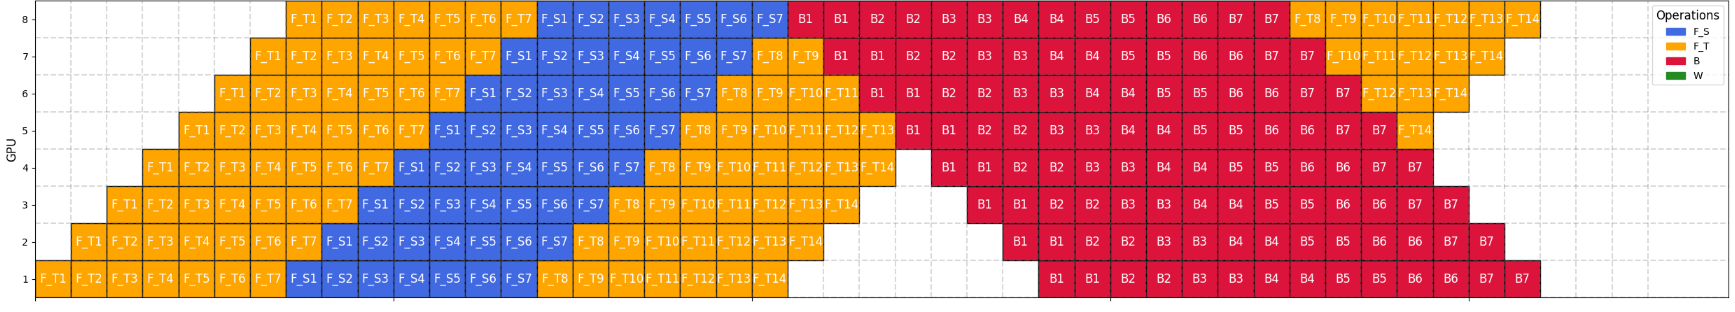
\includegraphics[width=\linewidth]{res/tspipe_8gpus.png}
  \caption{Sample figure caption.}
  \label{fig:tspipe}
\end{figure}

Frow this point forward, we consider $p$ to be the number of devices or GPUs and $m$ to be the number of microbatches where a microbatch is a subdivision of a batch. Furthermore, we consider that our batch size is the same for all strategies to be able to accurately determine the advantage of each. TSPipe states that for a given batch, it needs to be divided by $m=p-1$ to get $p-1$ microbatches. Moreover, TSPipe uses what was called a half backward, where the backward pass was done only half of the output at a time. By combining these two rules, we get the TSPipe schedule in Figure~\ref{fig:tspipe}.


The Figure~\ref{fig:tspipe} shows a full training iteration using TSPipe on a configuration of $8$ GPUs. As depicted by the Figure, TSPipe allows filling the idle time (pipeline bubble) with the next iteration teacher forwards. Nevertheless, it still can't fill the bubble of all iterations, which makes the schedule inefficient. Moreover, the half backward method is very rigid compared to the gradient decoupling method where the gradients with regard to activations and weights done separately and finally TSPipe forces the division of the batch by $p-1$ microbatches which is highly constraining.

% (this paragraph needs more explanation as to how rigid the half backward is and how is the p-1 microbatches constraining in terms of memory)

% - explain how TSPipe works.

% - drawbacks of using TSPipe.



\section{Methodology}
Our contribution aims to combine gradient decoupling and pipeline parallelism for knowledge distillation architectures such as RLHF algorithms. In this section, we describe the scheduling problem in hand and two scheduling strategies; one with $p-1$ microbatches as done in the TSPipe paper \cite{} and another that splits the batch into $2p$ microbatches or more similarly to what was used in the Zero-Bubble paper \cite{}. We focus mainly on high-level details in this section, leaving mathematical details to the Appendix ref\_section


% ZB + TS = ZBTS (Our contribution)

\subsection{Problem formulation}
In pipeline parallelism, all models are considered a sequence of blocks, where each block's output is the input of another and is assigned to a specific GPU. Given a fixed size batch, it is divided into $m$ microbatches to allow parallel execution, for example, once the first GPU completes the forward pass on the first microbatch it sends its output to the next GPU to allow it to start performing the forward pass while the first GPU start doing the forward pass of the next microbatch.


The global execution order is defined by a schedule, which specifies for each GPU the order of computations (forward and backward) on different microbatches. In this work we propose the combination of Knowledge Distilation (KD) architecture which emerge from studying famous RLHF algorithms and the gradient decoupling which was first introduced in the Zero-Bubble paper \cite{}. These two additions change the number of operation and introduces new inter-GPU and intra-GPU rules.


In the classical setting, only one type of forward computation exists. However, in Knowledge Distillation-like (KD) architectures two types of model forwards are used: a student model forward and a teacher model forward, which we denote respectively as $F_S$ and $F_T$. The only difference between these two forwards is that the activations of the student model are stored, while those belonging to the teacher model aren't. Additionally, the use of gradient decoupling splits the backward pass into two distinct steps : the B pass (computation of gradients w.r.t activations) and the W pass (computation of gradients w.r.t weights). Unlike the simple backward pass or the half backward pass used in TSPipe \cite{} which heavily depend on the backward pass of the previous stage, the decoupling offers two passes where only the B pass relies on the B pass of the previous GPU and the W pass can be done anytime after the corresponding B pass. Consequently, we have 4 types of computations to schedule, student forward, teacher forward, B pass and the W pass respectively noted as $F_S$, $F_T$, $B$ and $W$. It also important to note that although gradient decoupling offers more flexibility schedule-wise, it increases memory constraints as  the data required for operation W needs to be kept in memory for a longer time between B and W.


For a given GPU and a microbatch the order of operations is $F_S$ $\rightleftharpoons$ $F_T$, $B$, $W$, where $F_S$ and $F_T$ are interchangeable. We denote by $M_{F_S}$, $M_B$ \footnote{$M_{F_S}$ is usually greater than $M_B$, because actions for an entire model part is higher than gradients of output that form $M_B$} the amount of data kept in memory for one microbatch after operations $F_S$ and $B$ respectively \footnote{The passes $F_T$ and $W$ do not keep any data, therefore, $M_{F_T}=0$ and $M_W=0$}. Similarly, we denote by $T_{F_S}$, $T_{F_T}$, $T_B$ and $T_W$ the respective computation time of the operations $F_S$, $F_T$, $B$ and $W$ which we consider to be all equal according to the Zero-Bubble paper \cite{}. Additionally, we set $T$ to be the constant time needed to do a pass on the entire batch and $M_{F_S}^{Batch}$ and $M_B^{Batch}$ the amount of data kept after operation $F_S$ and $B$ respectively on the entire batch. Therefore, $T_{F_S}=T_{F_T}=T_B=T_W=\frac{T}{m}$, $M_{F_S}=M_{F_S}^{Batch}/m$ and $M_B=M_B^{Batch}/m$. However, in most cases the time of a teacher forward differs from the time of the student forward due to optimization and model size characteristics. Consequently, we set $T_{F_T} = \alpha T_{F_S},~~\alpha \in \mathbb{R}$, which gives us $T_{F_S}=T_B=T_W=\frac{T}{m}$, $T_{F_T}=\alpha \frac{T}{m}$, $M_{F_S}=M_{F_S}^{Batch}/m$ and $M_B=M_B^{Batch}/m$.


We formulise the schedule with gradient decoupling and a teacher student teacher architecture, which we named Zero Bubble Teacher Student (ZBTS), as an optimisation problem under linear constraints. We consider a sequential language model, partitioned into $p$ stages and a fixed-size batch sharded into $m$ microbatches. Two configurations emerge after a thorough study of the TSPipe paper \cite{} and the Zero-Bubble paper \cite{}. TSPipe uses $p-1$ microbatches with $p-1$ warm up teacher forwards, while Zero-Bubble proposes schedules using $2p$ microbatches or more for a true zero bubble pipeline parallelism. Therefore, we explore the two configurations \textbf{ZBTS$_{p-1}$} and \textbf{ZBTS$_{\ge 2p}$}, and prove their optimality using ILP solvers to find the best schedule that minimises the training time and respects the memory limits of individual GPUs.




\paragraph{Handcrafted schedule of ZBTS$_{p-1}$}

% \begin{figure}
%   \centering
%   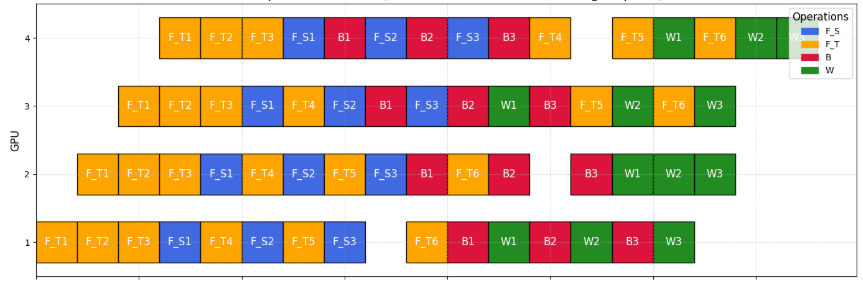
\includegraphics[width=0.8\linewidth]{res/solver_zbts_p-1_3p2m.png}
%   \caption{Sample figure caption. (This schedule will be modified)}
%   \label{fig:zbts_3}
% \end{figure}

\begin{figure}
  \centering
  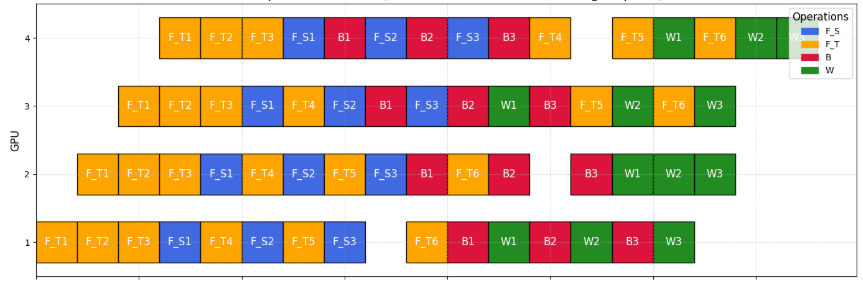
\includegraphics[width=0.8\linewidth]{res/solver_zbts_p-1_3p2m.png}
  % \fbox{\rule[-.5cm]{0cm}{4cm} \rule[-.5cm]{4cm}{0cm}}
  \caption{Handcrafted ZBTS$_{p-1}$ schedule for $p=4$ GPUs, $m=p-1=3$, $T=10$, $\alpha = 1$.}
  \label{fig:zbts_hand_3}
\end{figure}


Similarly to TSPipe, ZBTS$_{p-1}$ requires $p-1$ microbatches and $p-1$ warmup teacher forwards, to be able to reduce the bubble in the pipeline iterations.

We developed a handcrafted schedule that as shown in Figure~\ref{fig:zbts_hand_3}. This handcrafted strategy follows a structured set of rules: it begins with $p-1$ teacher forwards across all GPUs, followed by student forwards spaced by one  B pass time ($T_B$). B passes are then executed as soon as possible, followed immediately by W passes. Finally, any remaining computational bubbles are filled with the teacher forwards of the next iteration.


\paragraph{ILP schedule of ZBTS$_{\ge 2p}$}


\begin{figure}
  \centering
  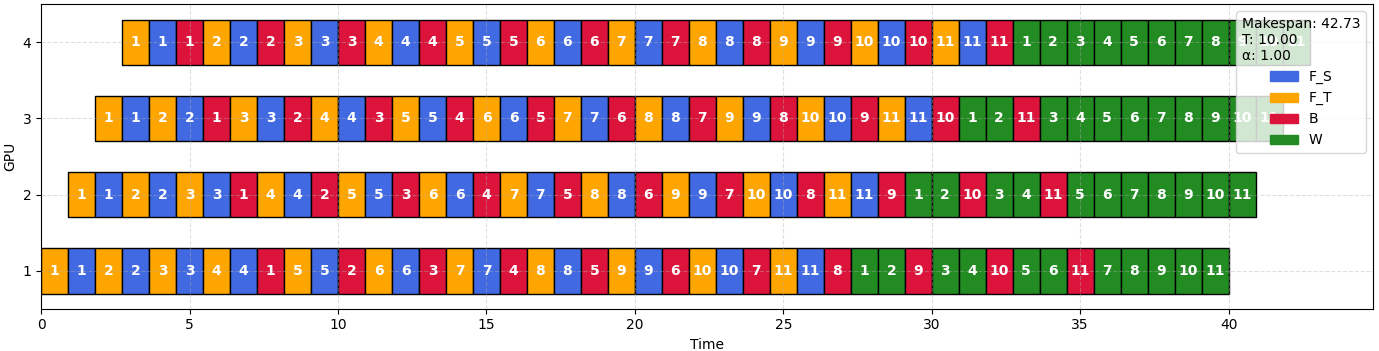
\includegraphics[width=\linewidth]{res/zbts_2p_4.png}
  \caption{Handcrafted ZBTS$_{\ge 2p}$ schedule for $p=4$ GPUs ($2p=8$), $m=11 \ge 8$, $T=10$, $\alpha = 1$.}
  \label{fig:zbts_hand_6}
\end{figure}

Unlike ZBTS$_{p-1}$ no warm up teacher forwards are needed nor for the first iteration not the intermediate iterations of the bubble since adopting $2p$ microbatches or more enables a true zero-bubble schedule. Given the fact that in the case of more than $2p$ microbatches we want to have repeatable pattern in the steady phase to be able to repeat it as many times as needed.

Therefore, we propose the handcrafted schedule strategy shown in Figure~\ref{fig:zbts_hand_6}, which is defined by a set of specific rules. The schedule begins by performing the teacher forward pass, immediately followed by the student forward pass for each microbatch. The B pass is then executed as soon as its dependencies are satisfied. Finally, once all forward passes are completed, the remaining computational bubble is filled with W passes. This simple set of rules provides an easy and flexible strategy allowing for a repeatable pattern in the steady phase of schedule, allowing as a consequence to increase easily the number of microbatches.

% - Schedule specification (doesn't require any warmup forwards)
% - Solver schedule doesn't work for $m>2p$, as a consequence, use handcrafted schedule that conserves memory limit and training time.




\section{Analytical evaluation}
So far we have studied three scheduling strategies that fall into the category of Knowledge Distillation (KD) architecture schedules, TSPipe (Baseline), ZBTS$_{p-1}$ and ZBTS$_{\ge 2p}$. To be able to precisely compare the schedules we need to test them under the same conditions and to use rigorous metrics that directly translate the efficiency and performance of a scheduling strategy. For the sake of transparency we considered arbitrary values for $M_{F_S}^{Batch}$, $M_B^{Batch}$ and $T$. It is mandatory to note that usually $M_{F_S}^{Batch} \ge M_B^{Batch}$ as explained previously, hence, we set $M_{F_S}^{Batch}=50~GB$, $M_B^{Batch}=20~GB$, $T=10~(units)$ and $\alpha \in \mathbb{R}$. For the sake of simplicity we tackle the case of $\alpha = 1$ first and leave other schedule cases in the appendix \ref{sec:appendix}.


\subsection{Metrics}
In the context of pipeline parallelism, scheduling strategies are traditionally evaluated using metrics that capture both time and resource efficiency. The primary metric is the makespan, defined as the total time to complete a single training iteration, which is directly proportional to the pipeline bubble size (idle time). A second critical metric is the peak memory consumption, representing the maximum memory load experienced by any GPU in the distributed environment, as this is often the bottleneck for model capacity. For a fixed batch size and consistent computation times per stage, the relationship between bubble size and makespan can be formalized.

To compute the peak memory we track the memory variation of all GPUs at every time step and accumulate the difference of memory after and before each operation ($F_S$, $F_T$, $B$ and $W$). During the teacher forward pass only the output of the model are stored which is negligible compared to the memory stored by activations or gradients, thus, $\Delta Memory(F_T)=0$. After performing the student forward pass the model part's activations are stored for that specific micorbatch used therfore $\Delta Memory(F_S)=M_{F_S}=M_{F_S}^{Batch}/m$. When it comes the B pass we free the memory allocated by the forward student pass and add the memory required by the data stored after the W pass, which gives us $\Delta Memory(B)=M_B- M_{F_S}=(M_B^{Batch}-M_{F_S}^{Batch})/m$. And finally in the W pass we desalocate the memory kept after the B pass such that $\Delta Memory(W)=-M_B=-M_B^{Batch}/m$.



\subsection{Comparison}
To evaluate the performance of our proposed schedules we compared their general formulas of makespan and peak memory to those of the TSPipe baseline.

\begin{figure}
  \centering
  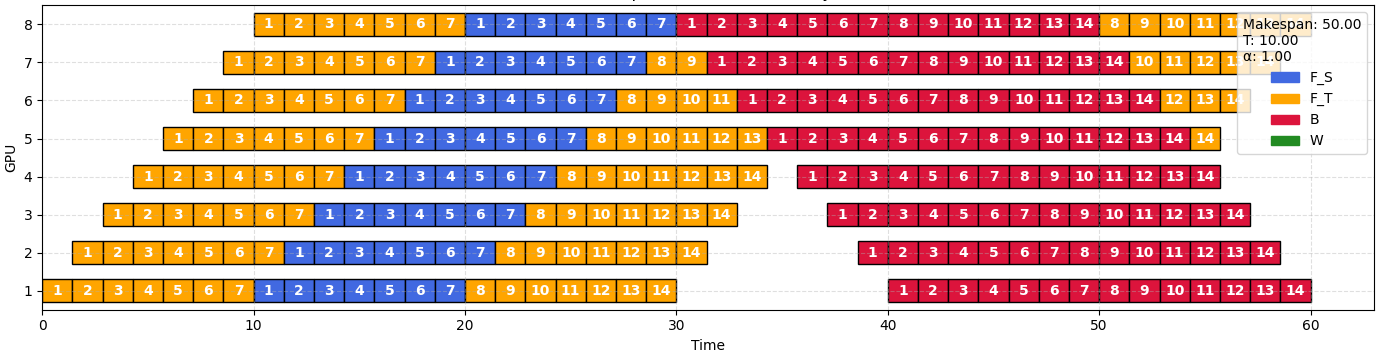
\includegraphics[width=\linewidth]{res/tspipe_8.png}
  % \fbox{\rule[-.5cm]{0cm}{4cm} \rule[-.5cm]{4cm}{0cm}}
  \caption{TSPipe for 8 GPUs.}
  \label{fig:tspipe_gen}
\end{figure}


\begin{equation}
    \text{makespan}_{\text{TSPipe}} = (p-1)(T_{F_S} + 2T_{F_T} + 2T_B)=(p-1)\cdot 5\cdot \frac{T}{p-1} = 5T
    \label{eq:mkspn_tspipe}
\end{equation}

\paragraph{TSPipe} Given that TSPipe is the baseline schedule that combines a teacher student architecture and the pipeline parallelism distribution method, it mandatory to determine its theoretical makespan and peak memory first. We consider an random intermediate iteration containing $m=p-1$ micorbatches as shown in Figure~\ref{fig:tspipe_gen}. The makespan of TSPipe is the time taken in the first GPU from the student forward of the first microbatch to the last backward pass of the last microbatch. According to Figure~\ref{fig:tspipe_gen} we can determine the makepsan by accumulating the time to perform $p-1$ student forwards, two times $p-1$ teacher forwards where the second $p-1$ teacher forward cells are filled with a pipeline bubble and finally, $2(p-1)$ half backward. Given the fact that gradient decoupling split the backward pass into a B and W pass of equal time stated before ($T_{backward} = T_B + T_W$). We consider the time to perform one half backward to be $T_B$. Consequently, we get the general $\text{makespan}_{\text{TSPipe}}$ formula in Equation~\ref{eq:mkspn_tspipe}.

\begin{equation}
    \text{PeakMem}_{\text{TSPpipe}}=(p-1)\frac{M_B^{batch}}{p-1} = M_B^{batch}
    \label{eq:peakmem_tspipe}
\end{equation}

When it comes to the peak memory of TSPipe, common machine learning knowledge states that activations are allocated during the forward pass until the adequate backward pass is computed. Along with the simulation in Figure~\ref{fig:tspipe_gen} the peak memory is reached when all student forwards are computed for each particular GPU. As a consequence, the peak memory of TSPipe can be denoted by the Equation~\ref{eq:peakmem_tspipe}.


\begin{figure}
  \centering
  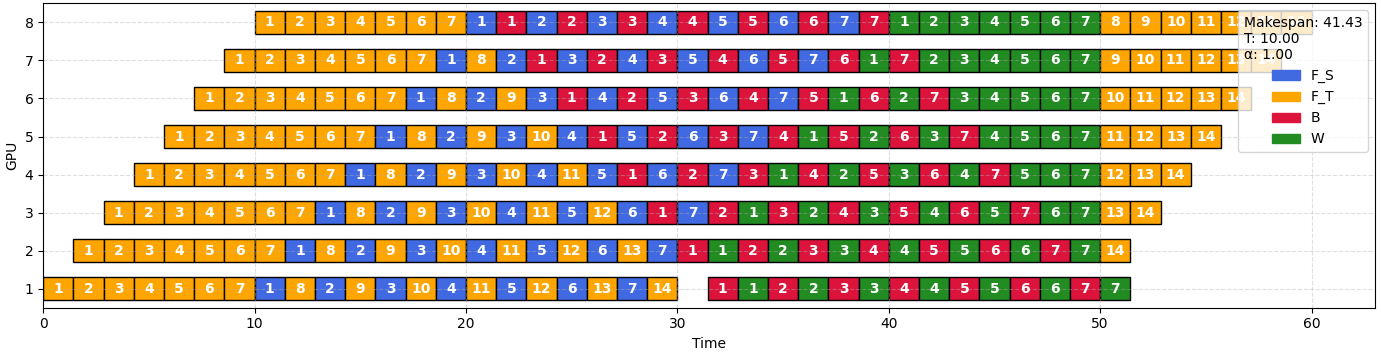
\includegraphics[width=\linewidth]{res/zbts_hand_p_1.png}
  % \fbox{\rule[-.5cm]{0cm}{4cm} \rule[-.5cm]{4cm}{0cm}}
  \caption{ZBTS$_{p-1}$ for 8 GPUs.}
  \label{fig:zbts_p_gen}
\end{figure}

\begin{equation}
    \text{makespan}_{\text{ZBTS}_{p-1}} = (p-1)(T_{F_T} + T_{F_S} + T_{B} + T_W) + T_{F_T} = (p-1) \cdot 4 \cdot \frac{T}{p-1} + \frac{T}{p-1} =4T + \frac{T}{p-1}
    \label{eq:makespan_zbts_p}
\end{equation}


\paragraph{ZBTS$_{p-1}$} Our first proposed solution based on ZBTS and uses the number of micorbatches specified in TSPipe ($m=p-1$), previously introduced as ZBTS$_{p-1}$, gives the intermediate iteration schedule in Figure~\ref{fig:zbts_p_gen} for $p=8$ GPUs. The Figure~\ref{fig:zbts_p_gen} shows that the makespan of ZBTS$_{p-1}$ is the time duration starting at the first student forward of the first microbatch and ending at the last W pass of the last microbatch. Given this information we can conclude that the training time for one iteration in the case of ZBTS$_{p-1}$ is the time needed to perform $p-1$ student forward, $p-1$ teacher forward, $p-1$ B passes, $p-1$ W passes and finally one additional bubble cell of time $T_{F_T}$. Therefore, the makespan of ZBTS$_{p-1}$ can be generalized as described in Equation~\ref{eq:makespan_zbts_p}.

\begin{equation}
    \text{PeakMem}_{\text{ZBTS}_{p-1}}=(p-1)\frac{M_B^{batch}}{p-1} = M_B^{batch}
    \label{eq:peakmem_zbts_p}
\end{equation}


Concerning the peak memory ZBTS$_{p-1}$, we have stated previously and formalised the memory impact of allocated data after each operation allowing us to precisely predict the peak memory of ZBTS$_{p-1}$. We performed a simulation tracking the memory variation after each pass for all GPUs, leading us to the fact that the first GPU reaches the peak memory of the schedule after performing all student forwards (i.e $p-1$ student forwards). Resulting in the general peak memory formula in Equation~\ref{eq:peakmem_zbts_p}.



\begin{figure}
  \centering
  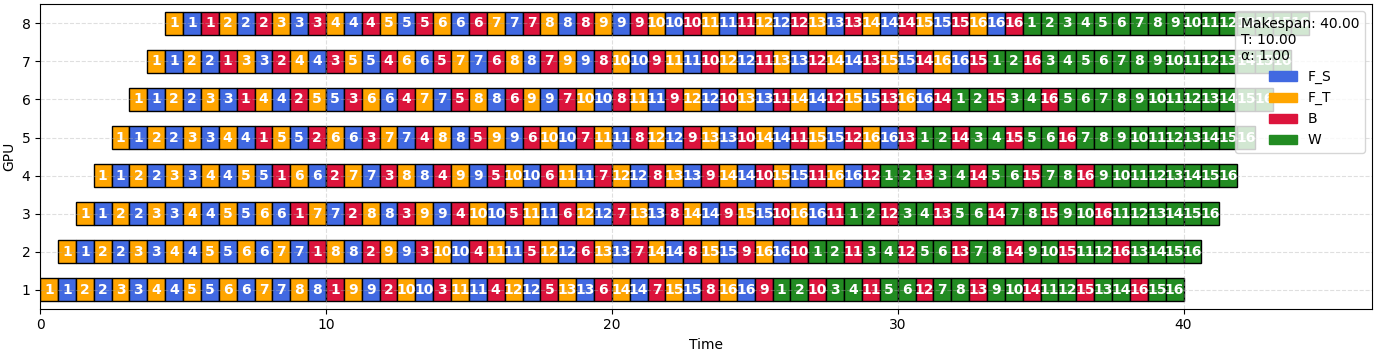
\includegraphics[width=\linewidth]{res/zbts_hand_2p.png}
  % \fbox{\rule[-.5cm]{0cm}{4cm} \rule[-.5cm]{4cm}{0cm}}
  \caption{ZBTS$_{\ge 2p}$ for 8 GPUs.}
  \label{fig:zbts_2p_gen}
\end{figure}

\begin{equation}
    \text{makespan}_{\text{ZBTS}_{\ge 2p}} = m(T_{F_T} + T_{F_S} + T_{B})+m ~ T_W=4m\frac{T}{m}=4T
    \label{eq:makespan_zbts_2p}
\end{equation}

\paragraph{ZBTS$_{\ge 2p}$} The second scheduling strategy we proposed, is based on the core ZBTS schedule type, combining gradient decoupling and a teacher student architecture, but uses $2p$ microbatches or more where $p$ is the number of GPUs and no warm up teacher forwards in contrasty to what is done in TSPipe and ZBTS$_{p-1}$. In ZBTS$_{\ge 2p}$ all the iterations are similar, unlike TSPipe and ZBTS$_{p-1}$ where the first and last iterations are different from the intermediate iterations in terms of number of teacher forwards.

Given the proposed schedule of the handcrafted ZBTS$_{\ge 2p}$ we get the Figure~\ref{fig:zbts_2p_gen} for $m=2p$ microbatches and $p=8$ GPUs. The figure depicts how the makespan for all GPUs is the same and it is the time between the first teacher forward of the first microbatch and the last W pass of the last microbatch. For instance, in the last GPU we observe a repeated pattern of $F_T \xrightarrow{} F_S \xrightarrow{} B$ done number of microbatches times ($m=2p$), followed by $m$ W passes. Thus the makespan of ZBTS$_{\ge 2p}$ is the time required to perform $m$ teacher forwards, $m$ student forwards, $m$ B passes, by following the pattern introduced previously, and $m$ W passes. This allows us to conclude that the makespan of ZBTS$_{\ge 2p}$ follows the Equation~\ref{eq:makespan_zbts_2p}.


\begin{figure}
  \centering
  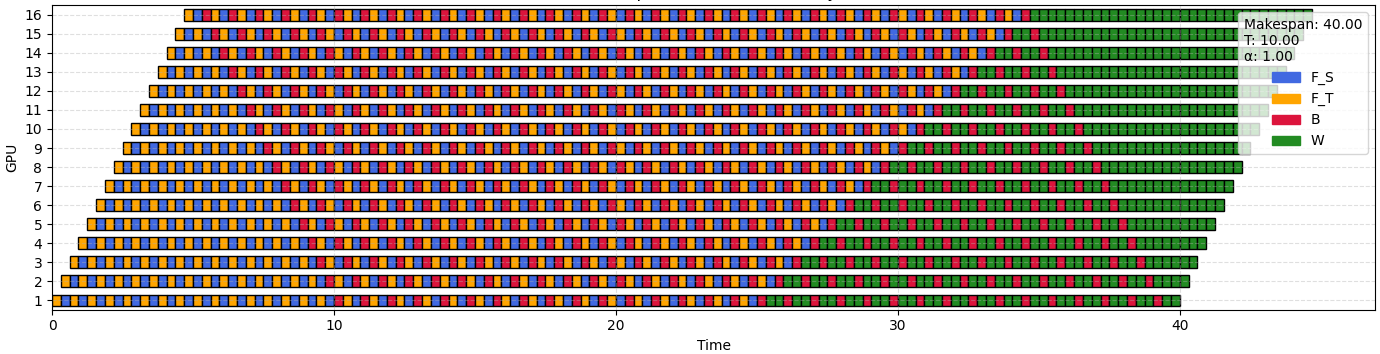
\includegraphics[width=\linewidth]{res/zbts_hand_2p_16.png}
  % \fbox{\rule[-.5cm]{0cm}{4cm} \rule[-.5cm]{4cm}{0cm}}
  \caption{ZBTS$_{\ge 2p}$ for 16 GPUs intermediate iteration to show number of wamrup student forwards.}
  \label{fig:zbts_2p_gen_16}
\end{figure}

\begin{equation}
    \text{PeakMem}_{\text{ZBTS}_{\ge 2p}}=\frac{(p-1)M_{F_S}^{batch} + (m-(p-1))M_B^{batch}}{m},~~~~~m\ge 2p
    \label{eq:peakmem_zbts_2p}
\end{equation}

In terms of peak memory performance, a clear high use of GPU memory was observed on the first GPU due to the multiple warm up student forwards done before reaching the steady phase with the $F_T \xrightarrow{} F_S \xrightarrow{} B$ pattern. As stated previously, a student forward introduces a positive allocated memory variation $\Delta Memory(F_S)=M_{F_S}^{Batch}/m$, a B pass adds a negative memory impact quantified by $\Delta Memory(B)=(M_B^{Batch}-M_{F_S}^{Batch})/m$ and finally, the teacher forward has a null allocated memory effect, $\Delta Memory(F_T)=0$. Hence we can determine the memory difference introduced by the steady phase pattern $\Delta Memory(F_T \xrightarrow{} F_S \xrightarrow{} B) = \sum_{op~\in~\{F_T,F_S,B\}} \Delta Memory(op) = M_B^{Batch}/m$.

The task now is to determine the number of times $x$ the warm up student forwards are done and the number of times $y$ the steady phase pattern is done $\text{PeakMem}_{\text{ZBTS}_{\ge 2p}} = x\Delta Memory(F_S) + y \Delta Memory(F_T \xrightarrow{} F_S \xrightarrow{} B)$. As mentioned before, the number of microbatches only affects the steady phase therefore the number of warm up student forwards is independent w.r.t number of micorbatches $m$. To be able to precisely determine the number of warm up students required for a ZBTS$_{\ge 2p}$ schedule simulated another schedule with $p=16$ GPUs as shown in Figure~\ref{fig:zbts_2p_gen_16}. Given Figure~\ref{fig:zbts_2p_gen_16} we have noticed that for $p$ GPUs, ZBTS$_{\ge 2p}$ requires $x=p-1$ warm up student forwards, therefore, $y=m - (p-1)$ steady phase patterns ($F_T \xrightarrow{} F_S \xrightarrow{} B$). Consequently, we get the general formula of the peak memory of ZBTS$_{\ge 2p}$ in Equation~\ref{eq:peakmem_zbts_2p}.

% ZBTS$_{\ge 2p}$: Achieves zero bubble, makespan = theoretical minimum, peak memory decreases with more microbatches.

\begin{table}[h]
\centering
\caption{Comparison of scheduling techniques for teacher-student architecture with $\alpha = 1$}
\label{tab:comparison}
\begin{tabular}{lccc}
\hline
\textbf{Schedule} & \textbf{Microbatches} & \textbf{Makespan} & \textbf{Peak Memory} \\
\hline
TSPipe & $p-1$ & $5T$ & $M_B^{batch}$ \\
ZBTS$_{p-1}$ & $p-1$ & $4T + \frac{T}{p-1}$ & $M_B^{batch}$ \\
ZBTS$_{\ge 2p}$ & $\ge 2p$ & $4T$ & $\frac{(p-1)M_{F_S}^{batch} + (m-(p-1))M_B^{batch}}{m}$ \\
\hline
\end{tabular}
\end{table}


\paragraph{Overall Comparison} As summarized in Table~\ref{tab:comparison}, 
...


\section{Conclusion}
ZBTS improves over TSPipe in both makespan and memory trade-offs.

With $p-1$ microbatches, makespan gains appear only when $p>2$ while the peak memory is the same.

With >=2p microbatches, ZBTS achieves true zero-bubble scheduling and reduced peak memory.



%%%%%%%%%%%%%%%%%%%%%%%%%%%%%%%%%%%%%%%%%%%%%%%%%%%%%%%%%%%%

\appendix
\label{sec:appendix}

\section{The effect of $\alpha$}
Even though the value of $\alpha$ changes the values of the makespan for every schedule, it does not change the general formulas of peak memory previously formulated.
To observe the effect of the value of $\alpha$ we propose to give three schedules for each strategy for values of $\alpha \in \{0.7,~1.7\}$


\begin{figure}
\centering
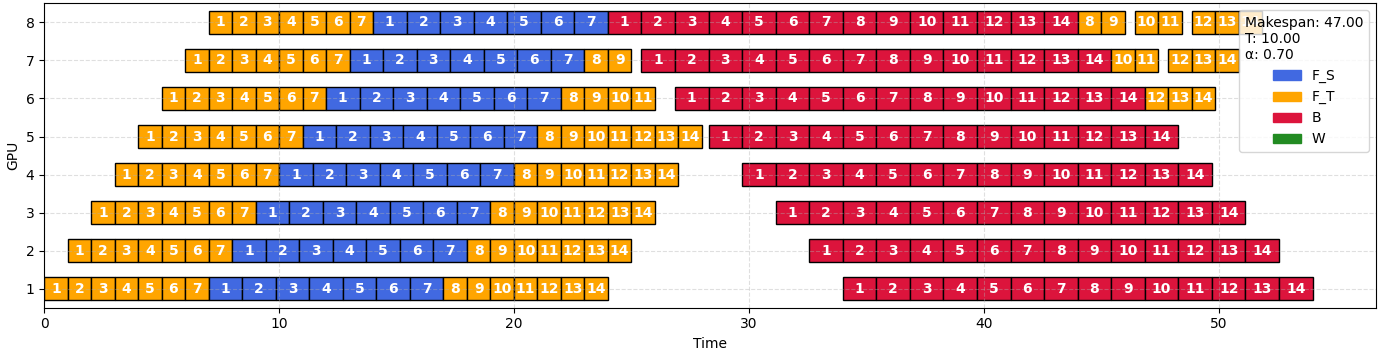
\includegraphics[width=\linewidth]{res/alpha_07_schedule_tsipe.png}
\caption{TSPipe with $\alpha = 0.7$.}
\label{fig:alpha_07_schedule_a}
\end{figure}

\begin{figure}
\centering
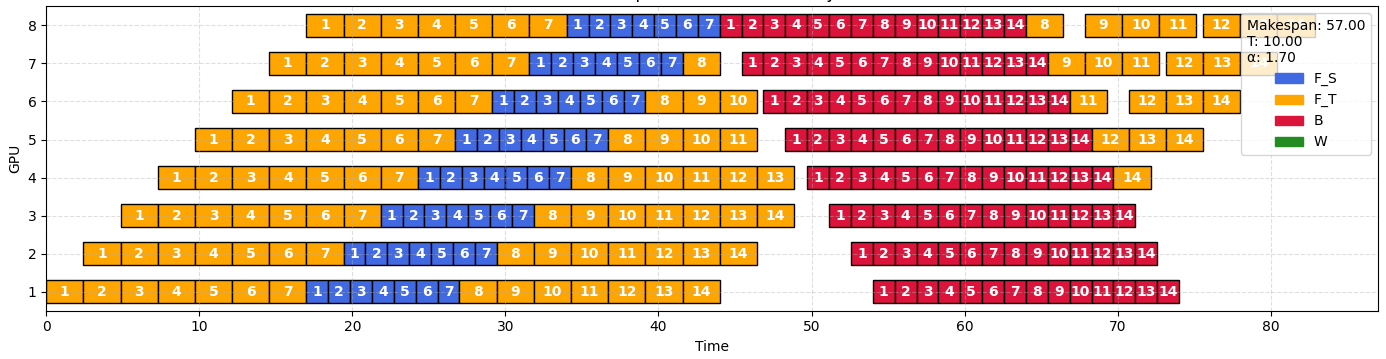
\includegraphics[width=\linewidth]{res/alpha_17_schedule_tspipe.png}
\caption{TSPipe with $\alpha = 1.7$.}
\label{fig:alpha_17_schedule_a}
\end{figure}

\begin{figure}
\centering
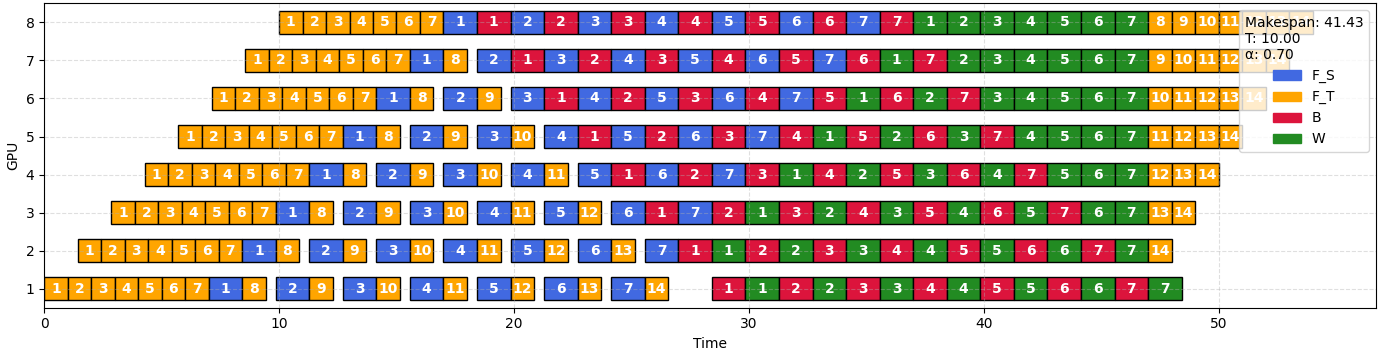
\includegraphics[width=\linewidth]{res/alpha_07_schedule_zbts_p_1.png}
\caption{ZBTS$_{p-1}$ with $\alpha = 0.7$.}
\label{fig:alpha_07_schedule_b}
\end{figure}

\begin{figure}
\centering
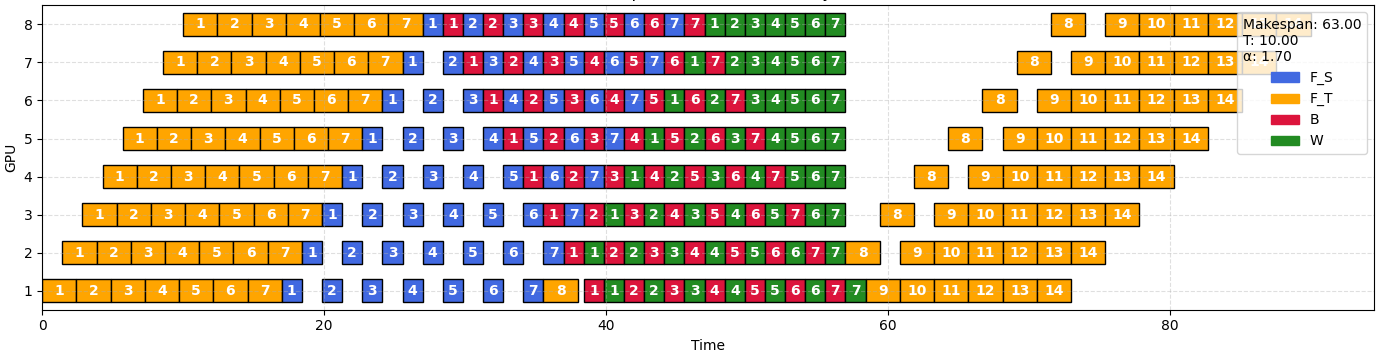
\includegraphics[width=\linewidth]{res/alpha_17_schedule_zbts_p_1.png}
\caption{ZBTS$_{p-1}$ with $\alpha = 1.7$.}
\label{fig:alpha_17_schedule_b}
\end{figure}

\begin{figure}
\centering
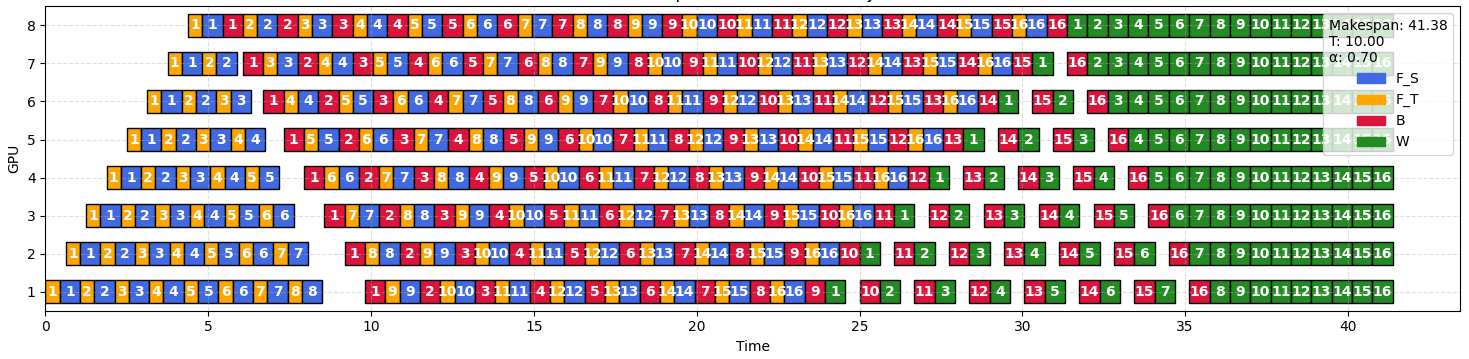
\includegraphics[width=\linewidth]{res/alpha_07_schedule_zbts_2p.png}
\caption{ZBTS$_{\ge 2p}$ with $\alpha = 0.7$.}
\label{fig:alpha_07_schedule_c}
\end{figure}

\begin{figure}
\centering
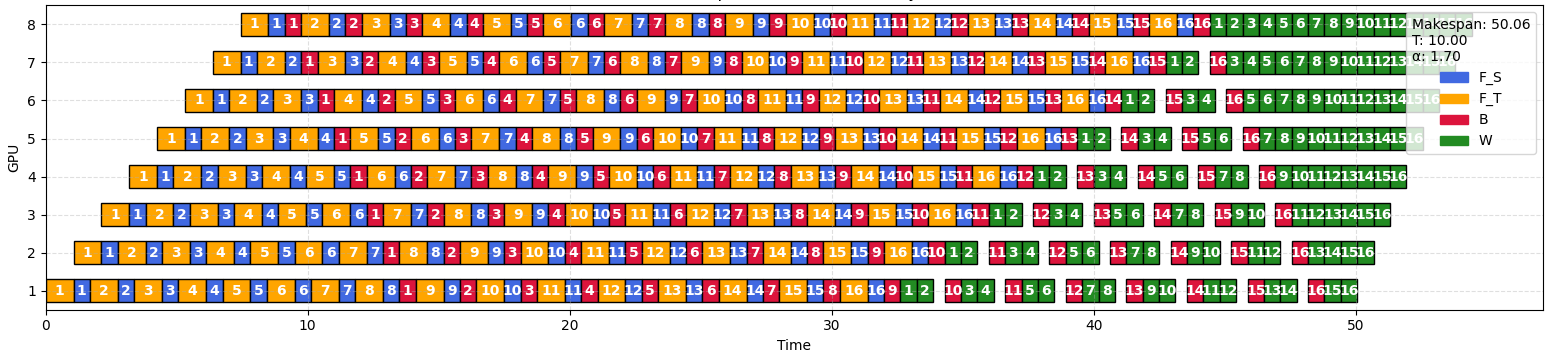
\includegraphics[width=\linewidth]{res/alpha_17_schedule_zbts_2p.png}
\caption{ZBTS$_{\ge 2p}$ with $\alpha = 1.7$.}
\label{fig:alpha_17_schedule_c}
\end{figure}

\newpage 
The previously depicted schedules sole goal is to simplify the imagination of the schedule for different values of $\alpha$ however multiple behaviours emerge for each particular schedule. Therefore we propose to plot the makepsan for each scheduling strategy with regard to $\alpha$ values.

\begin{figure}[ht!]
\centering
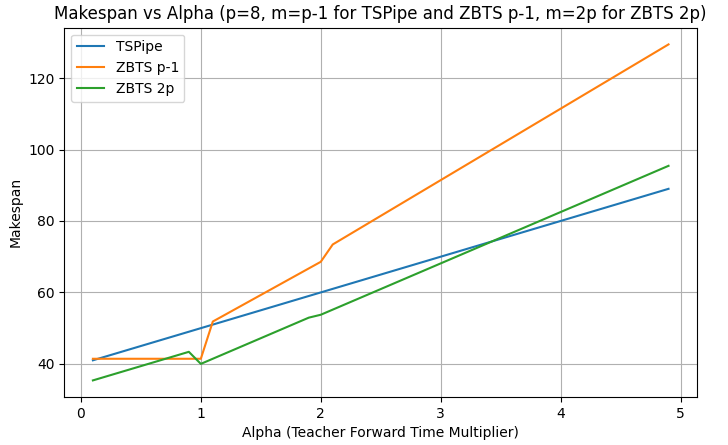
\includegraphics[width=0.8\linewidth]{res/makespan_8.png}
\caption{Makespan comparison for all schedules (p=8 GPUs, m=2p for ZBTS$_{\ge 2p}$) }
\label{fig:makespan_comp_8}
\end{figure}

We start by comparing the makespan of all schedule for 8 GPUs and values of alpha ranging from $0.1$ to $5$ as shown in figure~\ref{fig:makespan_comp_8}. We notice a change in makespan evolution, for ZBTS$_{p-1}$ and ZBTS$_{\ge 2p}$, at multiple transitions in alpha values one at $\alpha=1$ and one at $\alpha=2$.

\begin{figure}[ht!]
\centering
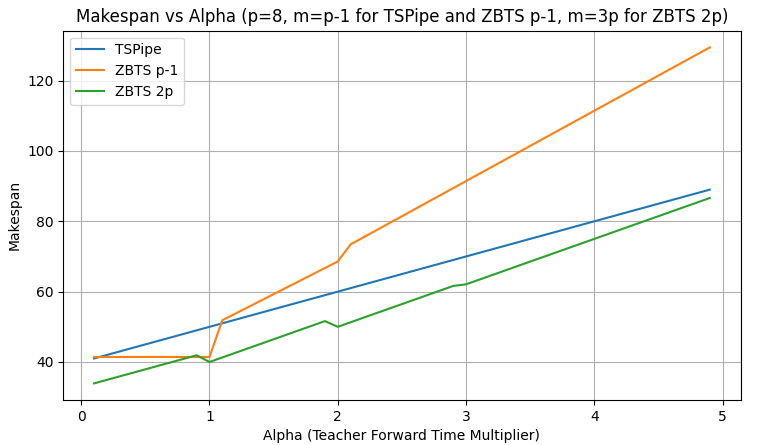
\includegraphics[width=0.8\linewidth]{res/makespan_8_3p.png}
\caption{Makespan comparison for all schedules (p=8 GPUs, \textbf{m=3p} for ZBTS$_{\ge 2p}$) }
\label{fig:makespan_comp_8_3p}
\end{figure}

Given the fact that the only scheduling strategy that has the flexibility to change its number of microbatches is ZBTS$_{\ge 2p}$, we plot the evolution of makespan for ZBTS$_{\ge 2p}$ with $m=3p$, resulting in figure~\ref{fig:makespan_comp_8_3p}.


\newpage
\section{Integer Linear Programming Formulation}

We propose an ILP formulation to find the optimal schedule for a teacher-student architecture, building upon the approach used in the Zero Bubble paper. We start by providing the notations and the core formulation.

\subsubsection{Notations and Formulation}

The input values of the ILP formulation use the following notations:
\begin{itemize}
    \item $p$ is the number of stages (GPUs), indexed with $i$;
    \item $m$ is the number of microbatches, indexed with $j$;
    \item $c \in \{F_S, F_T, B, W\}$ is used to index the operation type among: student forward, teacher forward, backward w.r.t. inputs, and backward w.r.t. parameters (weight gradients);
    \item $T_{\text{comm}}$ is the communication time between GPUs;
    \item $M_{\text{limit}}$ is the available memory of each GPU.
\end{itemize}

For a specific operation $c$ in stage $i$ on microbatch $j$, we define the following variables:
\begin{itemize}
    \item $T_{i,j,c}$ is the duration of the operation,
    \item $E_{i,j,c}$ is the ending time of the operation,
    \item $S_{i,j,c}$ is the start time of the operation, with $E_{i,j,c} = S_{i,j,c} + T_{i,j,c}$.
\end{itemize}

Furthermore, we define $\Delta M$ the memory difference caused by an operation as:
\[
\begin{aligned}
&\Delta M(i, j, F_T) = 0 \\
&\Delta M(i, j, F_S) = M_{F_S}, \\
&\Delta M(i, j, B~)~ = M_B - M_{F_S}, \\
&\Delta M(i, j, W) ~= -M_B.
\end{aligned}
\]

We define the ILP formulation for ZBTS$_{\ge 2p}$ ($m\ge2p$) as:
\begin{align}
    \text{min.} & \quad \max_{i \in [1,p]} E_{i,m,W} - \min(S_{i,1,F_T}, S_{i,1,F_S}) \label{eq:objective} \\
    \text{s.t.}~~~~~~~~E_{i,j,c} & = S_{i,j,c} + T_{i,j,c} \quad \forall i, j, c \label{eq:time_relation} \\
    S_{i,j,B} & \geq \max(E_{i,j,F_S}, E_{i,j,F_T}) \quad \forall i, j \label{eq:forward_backward} \\
    S_{i,j,W} & \geq E_{i,j,B} \quad \forall i, j \label{eq:backward_weight} \\
    S_{i,j,c} & \geq E_{i,j-1,c} \quad \forall i, c, j \in [2, m] \label{eq:microbatch_order} \\
    S_{i,j,F_S} & \geq E_{i-1,j,F_S} + T_{\text{comm}} \quad \forall i \in [2, p], j \label{eq:forward_comm_s} \\
    S_{i,j,F_T} & \geq E_{i-1,j,F_T} + T_{\text{comm}} \quad \forall i \in [2, p], j \label{eq:forward_comm_t} \\
    S_{i,j,B} & \geq E_{i+1,j,B} + T_{\text{comm}} \quad \forall i \in [1, p-1], j \label{eq:backward_comm} \\
    E_a & \geq E_b + T_a - y_{(a,b)} \cdot \mathcal{M} \quad \forall a,b \in \text{tasks of same stage } i \label{eq:precedence1} \\
    E_b & \geq E_a + T_b - y_{(b,a)} \cdot \mathcal{M} \quad \forall a,b \in \text{tasks of same stage } i \label{eq:precedence2} \\
    M_{\text{limit}} & \geq \sum_{a} \Delta M(a) \cdot y_{(a,b)} \quad \forall a,b \in \text{tasks of same stage } i \label{eq:memory_constraint}
\end{align}


% We define the ILP formulation for ZBTS$_{p-1}$ ($m=p-1$) as:
% \begin{align}
%     \text{min.} & \quad \max_{i \in [1,p]} E_{i,m,W} - \min(S_{i,\textbf{p-1},F_T}, S_{i,1,F_S}) \label{eq:objective} \\
%     \text{s.t.}~~~~~~~~E_{i,j,c} & = S_{i,j,c} + T_{i,j,c} \quad \forall i, j, c \label{eq:time_relation} \\
%     S_{i,j,B} & \geq \max(E_{i,j,F_S}, E_{i,j,F_T}) \quad \forall i, j \label{eq:forward_backward} \\
%     S_{i,j,W} & \geq E_{i,j,B} \quad \forall i, j \label{eq:backward_weight} \\
%     S_{i,j,c} & \geq E_{i,j-1,c} \quad \forall i, c, j \in [2, m] \label{eq:microbatch_order} \\
%     S_{i,j,F_S} & \geq E_{i-1,j,F_S} + T_{\text{comm}} \quad \forall i \in [2, p], j \label{eq:forward_comm_s} \\
%     S_{i,j,F_T} & \geq E_{i-1,j,F_T} + T_{\text{comm}} \quad \forall i \in [2, p], j \label{eq:forward_comm_t} \\
%     S_{i,j,B} & \geq E_{i+1,j,B} + T_{\text{comm}} \quad \forall i \in [1, p-1], j \label{eq:backward_comm} \\
%     E_a & \geq E_b + T_a - y_{(a,b)} \cdot \mathcal{M} \quad \forall a,b \in \text{tasks of same stage } i \label{eq:precedence1} \\
%     E_b & \geq E_a + T_b - y_{(b,a)} \cdot \mathcal{M} \quad \forall a,b \in \text{tasks of same stage } i \label{eq:precedence2} \\
%     M_{\text{limit}} & \geq \sum_{a} \Delta M(a) \cdot y_{(a,b)} \quad \forall a,b \in \text{tasks of same stage } i \label{eq:memory_constraint}
% \end{align}

% (-- add ILP formulation for TSPipe+ZB --)

The optimization objective in equation \ref{eq:objective} minimizes the makespan of the pipeline by reducing the difference between the completion time of the last W pass and the earliest start among the forward passes of the first microbatch. Constraint \ref{eq:time_relation} enforces consistency between start and end times of each task. Equations \ref{eq:forward_backward} and \ref{eq:backward_weight} force the order of operations: the backward pass must wait for both forward passes to finish, and the weight gradient pass can only start after the backward pass. Constraint \ref{eq:microbatch_order} ensures that for the same stage $i$ and pass $c$, the task of microbatch $j-1$ has to be done before that of microbatch $j$.

The inter-stage dependencies constraints are specified by equations \ref{eq:forward_comm_s} and \ref{eq:forward_comm_t}, where forward passes of stage $i$ cannot begin before the corresponding forward passes of stage $i-1$ are completed, and by equation \ref{eq:backward_comm}, which ensures that backward passes of stage $i$ cannot begin before the backward passes of stage $i+1$ are done. The constraints in equations \ref{eq:precedence1} and \ref{eq:precedence2} define precedence relationships between tasks within the same stage, guaranteeing no overlapping execution. Finally, the memory constraint in equation \ref{eq:memory_constraint} ensures that the cumulative memory usage of all tasks scheduled before a given task does not exceed the device memory limit $M_{\text{limit}}$.



We define the ILP formulation for ZBTS${p-1}$ ($m=p-1$) similarly to the ILP formulation of ZBTS$_{\ge 2p}$ but with a slight change in indexes.

\begin{itemize}
\item $i \in [1, p]$: stage index (GPU index)
\item For operations $c \in {F_S, B, W}$: $j \in [1, m]$ where $m = p-1$
\item For operation $F_T$ (teacher forward): $j \in [p, 2m]$ (i.e., $j \in [p, 2(p-1)]$) correspond to the extra teacher forwards from the next batch
\item Implementation note : in the ILP formulation of ZBTS$_{\ge 2p}$ the operation are performed in the order $F_S$ $\rightleftharpoons$ $F_T$, $B$, $W$, where $F_S$ and $F_T$ are interchangeable. But in the case of ZBTS${p-1}$ we drop $F_T$ from the order constraint since they are next batch teacher forwards.
\end{itemize}

%%%%%%%%%%%%%%%%%%%%%%%%%%%%%%%%%%%%%%%%%%%%%%%%%%%%%%%%%%%%



\end{document}